\subsection{Was bedeutet MOS-Technologie}
MOS steht für Metal Oxide Semiconductor.
Sie heißen auch unipolar: nur ein Ladungsträgertyp ist am Stromtransport beteiligt
	\subsubsection{NMOS/PMOS}
		NMOS bzw. PMOS sind nach der im Kanal entstehenden n- bzw. p-Leitung benannt.
	\subsubsection{CMOS}
		CMOS steht für Complementary MOS.
		Hierbei handelt es sich um eine kombinierte Verwendung von NMOS- und PMOS-Transistoren in einem Schaltkreis. Diese Anordnung ist stromsparend, hat eine geringe Verlustleistung und hoher Integrationsgrad.
\subsection{MOS-Kondensatoren}
	Die allgemeinere Bezeichung ist MIS-Kondensator. MIS - metal insulator semiconductor. Wobei der der Isolator  häufig aus Siliziumdioxid besteht
	\subsubsection{Grundaufbau}
	Der MOS-Kondensator besteht aus 
	\begin{itemize}
		\item Metallelektrode
		\item Isolator
		\item dotiertem Silizium		
	\end{itemize}	
	\begin{center}
		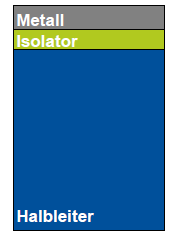
\includegraphics[width=0.2\linewidth]{Kapitel/Kap06/MOSKondensator}
	\end{center}
	
	\subsubsection{Flachbandfall}
		Background: im thermischen Gleichgewicht kommt es zu einem Ausgleich der unterschiedlichen Fermi-Niveaus (Halbleiter und Metall)
		\begin{itemize}
			\item Spannungsunterschied wird als Kontaktpotenzial bezeichnet
			\item 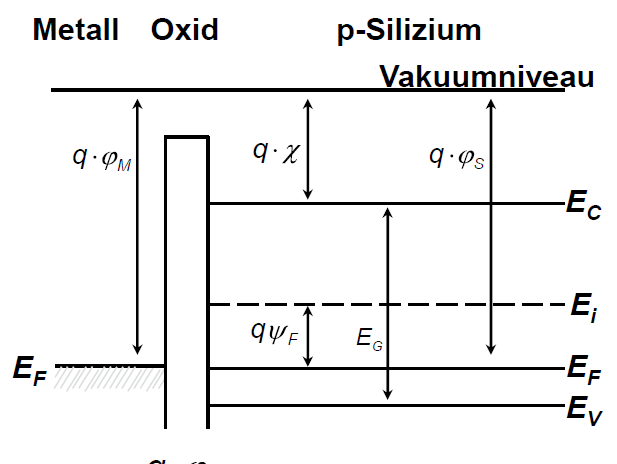
\includegraphics[width=0.4\linewidth]{Kapitel/Kap06/Kontaktpotential} 			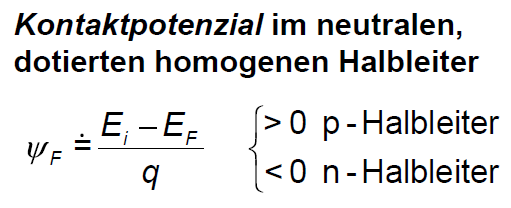
\includegraphics[width=0.4\linewidth]{Kapitel/Kap06/Kontaktpotential2}
			
			\item es bilden sich an der Grenzschicht zwischen Metall und Isolator positive und dem entgegengesetzt an der Grenzschicht zwischen Isolator und Halbleiter negative Ladungen aus.
			\item Es bildet sich eine Raumladungszone im Halbleiter			 		
		\end{itemize}
		Wichtig: Gleicht man das Kontaktpotenzial und den Spannungsabfall über das Oxid durch eine bestimmte schwache 	Vorspannung aus, so verschwindet die Raumladungszone man spricht vom Flachbandfall und der angelegten Flachbandspannung $U_{FB}$.
		
	\newpage
		
	\subsubsection{Anreicherung/Akkumulation, Verarmung, Inversion}
		Arbeitszustände (in diesen Fällen für für p-Silizium Substrate):
		\newline
		!!! Diagramme dienen nur der Veranschaulichung, Inversionsdiagramme sind wichtig !!!!
		\newline
		\textbf{Akkumulation:}
		\newline
		Beim Anlegen einer negative Spannung ($U_{MS} < 0 V $) gegenüber dem Substrat wandern die positiven Ladungsträger im Substrat zur 		Grenzschicht, sammeln sich dort und bilden eine Anreicherungszone
		\newline
		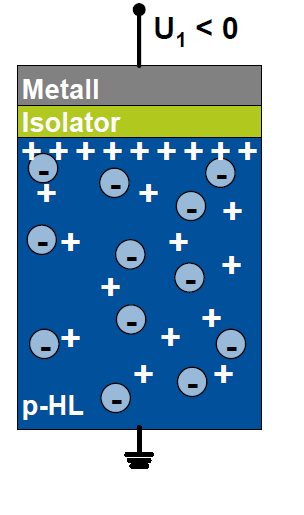
\includegraphics[width=0.25\linewidth]{Kapitel/Kap06/Akkumulation1}		
		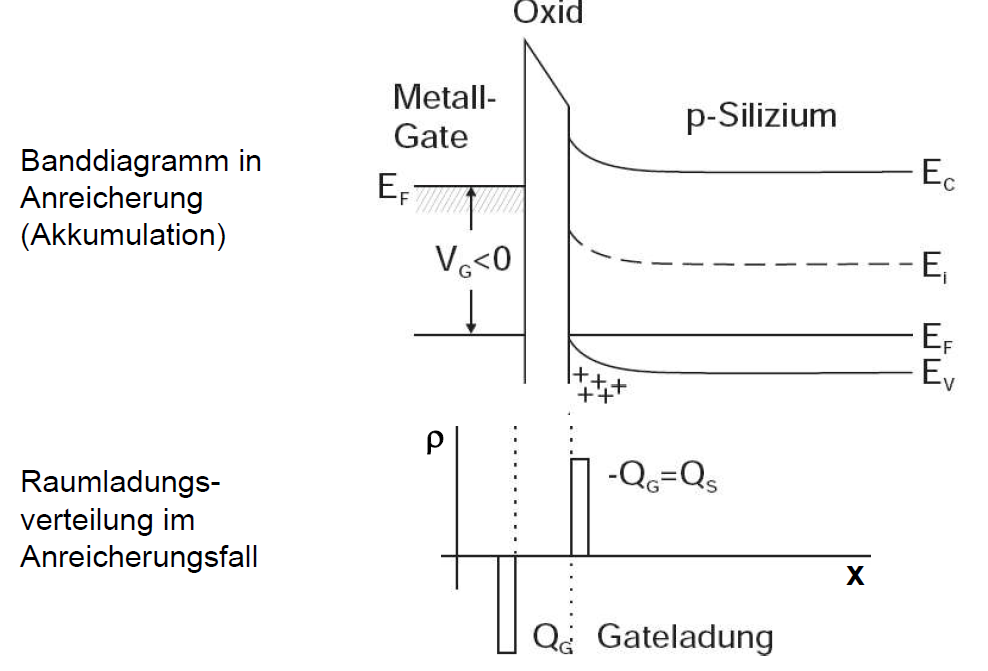
\includegraphics[width=0.60\linewidth]{Kapitel/Kap06/Akkumulation}
		\newline
		\newline
		
		\textbf{Verarmung:}
		\newline
		Bei Anlegen des Pluspols am Metall und
		des negativen Pols am Substrat ($U_{MS} > 0V$) wandern negative Ladungs-träger
		(Minoritäten) im Substrat an die Grenzschicht und rekombinieren mit den dort befindlichen freien positiven Ladungsträgern.
		\newline 
		In der Nähe der Grenzschicht entsteht durch die Rekombinationen eine 		Raumladungszone, die an freien 		Ladungsträgern verarmt ist. Diese Zone wird als Verarmungszone bezeichnet.
		\newline
		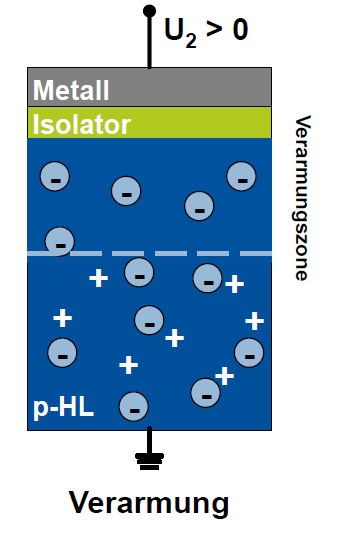
\includegraphics[width=0.25\linewidth]{Kapitel/Kap06/Verarmungszone1}
		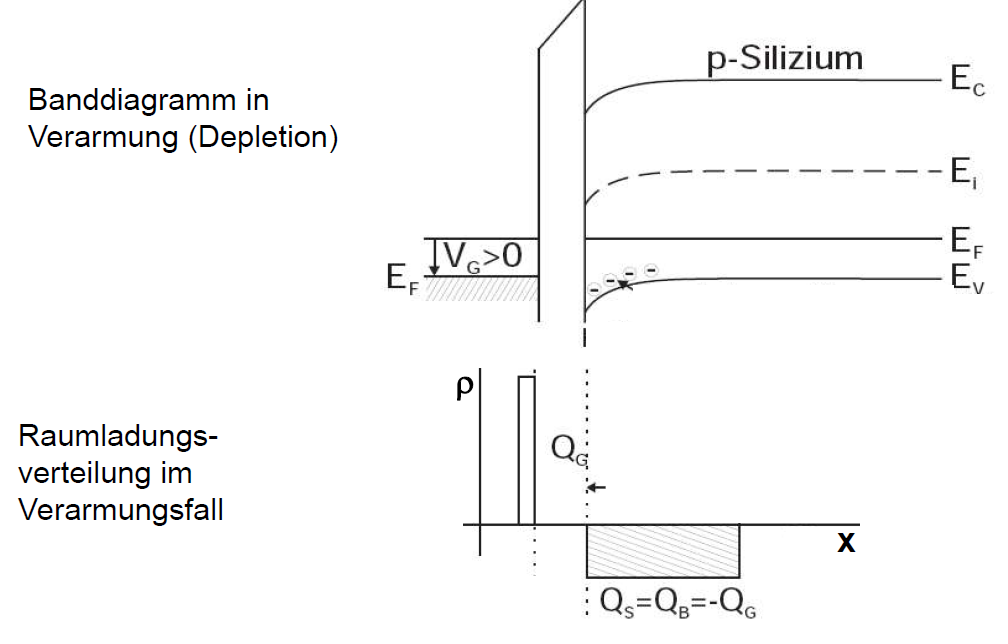
\includegraphics[width=0.60\linewidth]{Kapitel/Kap06/Verarmungszone2}
		
		\textbf{Inverstion:}
		\newline
		Überschreitet die angelegte Spannung eine Schwellspannung ($U_{MS} > U_{th}$ ,Threshold) bildet sich im ursprünglich p-dotierten Substrat ein n-dotiertes Gebiet. Es stehen keine freien Löcher mehr an der Grenzschicht zur Rekombination zur Verfügung.
		\newline
		Die so entstandene Zone, die die frei beweglichen negativen Ladungsträger enthält, wird als Inversionszone 	bezeichnet.
		\newline
		Hierbei unterscheidet man zwischen schwacher Inversion und starker Inversion.
		Bei starker Inversion entsteht im Halbleiter an der Grenze zum Isolator ein Elektronenkanal, in dem n-Leitung möglich ist
		\newline
		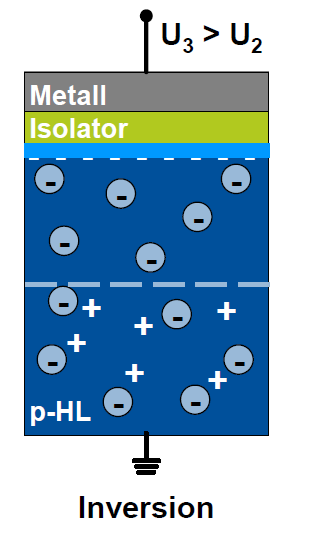
\includegraphics[width=0.25\linewidth]{Kapitel/Kap06/Inverstion1}		
		

		\textbf{Wichtige Graphiken zur Inversion:}
		\newline
		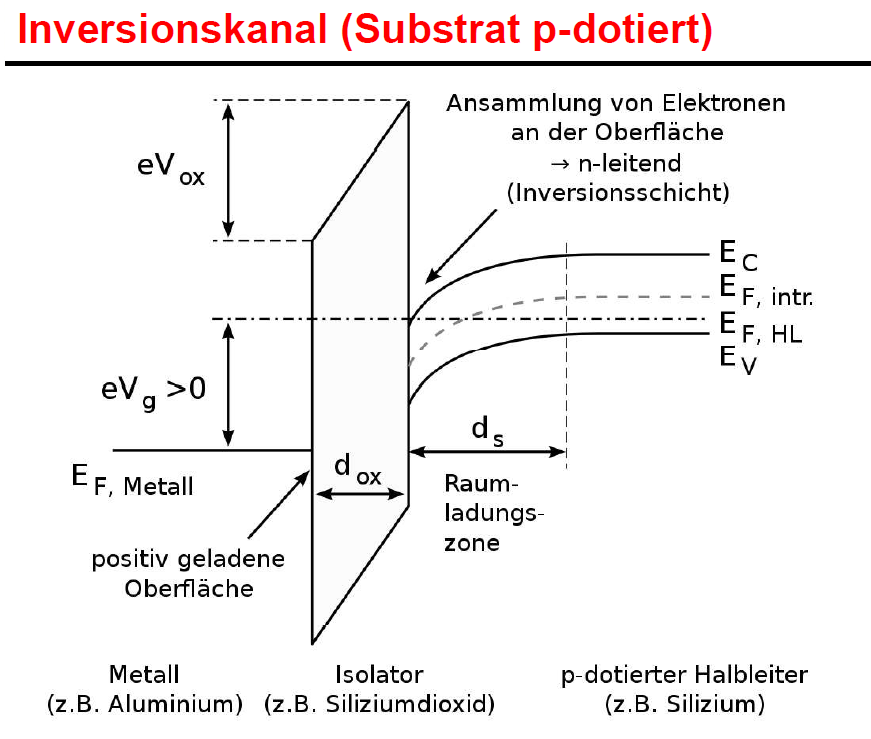
\includegraphics[width=0.5\linewidth]{Kapitel/Kap06/InversionPKanal}		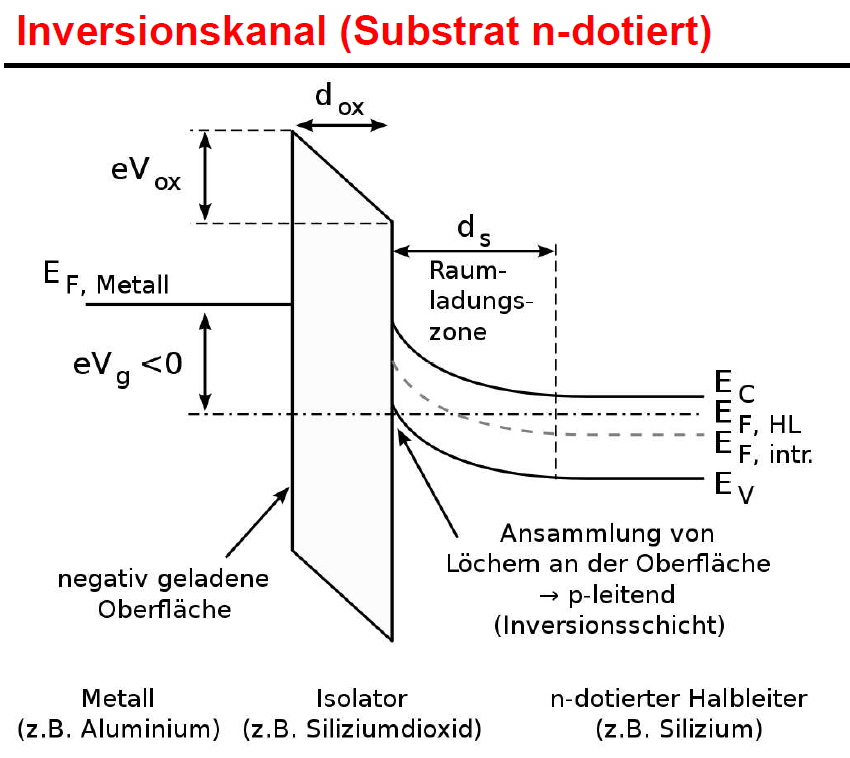
\includegraphics[width=0.48\linewidth]{Kapitel/Kap06/InversionNKanal}
		
		
	\newpage	
\subsection{MOS-Transitoren}
	MOS Transistoren sind Feldeffekttransistoren =
	MOSFET
	\newline
	Das Funktionsprinzip ist historisch gesehen schon länger bekannt (Patent Lilienfeld 1926) als der Bipolartransistor.
	
		Ein MOSFET ist ein aktives Bauelement mit mindestens drei Anschlüssen:
	\begin{itemize}
		\item S (source, dt. Quelle)
		\item D (drain, dt. Abfluss)
		\item G (gate, dt. Steuerelektrode)
		\item (B (bulk, dt. Substrat), Bei einigen Bauformen wird ein zusätzlicher Anschluss B nach außen geführt. Meistens ist das 		Substrat jedoch intern mit S verbunden )
	\end{itemize}
	Betrieb: Majoritätsladungsträger fließen von S nach D:
	\begin{itemize}
		\item unipolares Bauelement (nur ein Ladungsträgertyp bewegt sich)
		\item laterales Bauelement
	\end{itemize}
	
	\subsubsection{Grundaufbau}	
		
	\begin{itemize}
		\item Als Grundmaterial dient ein schwach p-dotierter Siliziumeinkristall (Substrat).
		\item In dieses Substrat sind zwei stark n-dotierte Gebiete eingelassen, die den Source- bzw. Drain-Anschluss erzeugen. Zwischen den beiden Gebieten befindet sich weiterhin
		das Substrat. So entsteht eine npn-Struktur
		\item Genau über diesem verbleibenden Zwischenraum befindet sich eine sehr dünne, widerstandsfähige Isolierschicht, das Gate-Dielektrikum das die darüberliegende Gate-Elektrode vom Silizium (genauer vom Kanalgebiet) trennt.
			\begin{itemize}
				\item Gatedielektrikum: Siliziumdioxid $SiO_2$ => hoch-K Materialien
				\item Gateelektrode: Ehemals: Aluminium, Heute: poly-Si => verschiedene Metalle
			\end{itemize}
	\end{itemize}
	Grundaufbau eine n-Kanal MOSFET:
	%MOS Transistor
	\begin{center}
		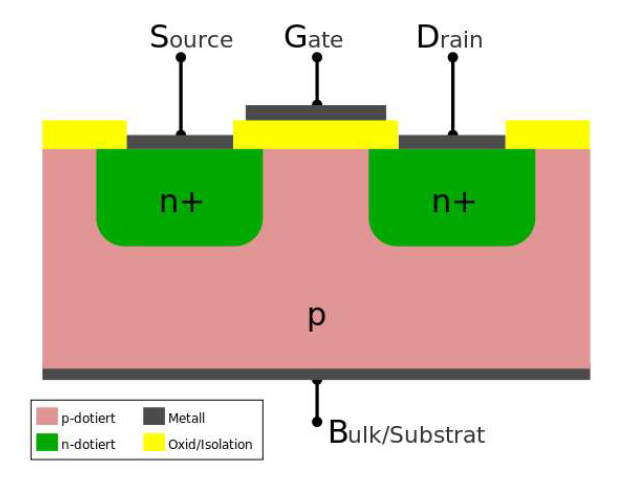
\includegraphics[width=0.5\linewidth]{Kapitel/Kap06/MOS_Transistor.png}
		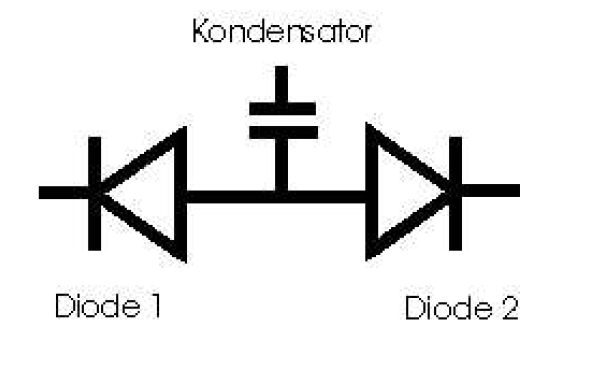
\includegraphics[width=0.2\linewidth]{Kapitel/Kap06/DiodenbildMOS}			
	\end{center}

	\subsubsection{Funktionsweise eines n-Kanal-Anreicherung-Transistoren}	
	Basierend auf dem Feldeffekt wird der Stromfluss wird durch ein an G anliegendes	elektrisches Feld gesteuert.
	\newline
	Gate-Anschluss, Dielektrikum und Bulk-Anschluss bilden einen (MOS-)Kondensator.
	Dieser kann in den drei oben beschriebenen Arbeitszuständen	Anreicherung, Verarmung und Inversion betrieben werden.
	Wird die Schwellspannung überschritten erreicht der n-MOS den Inversions-Zustand und das eigentlich p-dotierte Substrat wird nahe an der Isolierschicht n-leitend.
	\newline
	Die Geschwindigkeit ist vom Ladungsträgertransport von Source zum Drain abhängig. Dabei liegen die heutigen Kanallängen bei < 32 nm.
	\newline
	
	Der Typ ist jeweils nach dem Inversionskanal bezeichnet. Das Substrat ist immer entgegengesetzt dotiert:		
	\begin{itemize}
		\item P-MOS: Substrat=n
		\item N-MOS: Substrat=p
	\end{itemize}

	\subsection{Schwellspannung}
		Die Schwellspannung $U_{th}$ ist die Spannung, bei der bei einem Anreicherungstypen ein Kanal entsteht und bei einem Verarmungstypen der Kanal unterbrochen wird. 
		Die Schwellspannung hängt dabei Prozesstechnisch von der Dotierungen von Source, Drain und des Kanal-Gebietes ab.
	\subsubsection{neuere Entwicklungen}
		\textbf{Problem: }
		\newline
		Bei der Skalierung zu neuen Technologiegenerationen wird auch die Gateoxiddicke ebenfalls reduziert. 
		Die Tunnel/Leak-Ströme steigen exponentiell mit abnehmender Dicke.
		Irgendwann wäre man bei 3 Lagen von SiO2-Tetraedern. Die ist technisch nicht mehr homogen realisierbar (min. Schwankung 33 \%), da auch nicht mehr messbar. 
		\newline
		\textbf{Lösung: }
		\newline
		Daher muss trotz Skalierung das Dielektrikum dicker sein. Um die Kapazität bei größerer Dicke beizubehalten werden sogenannte High-K Dielektrika eingesetzt. 
		
		$C = \frac{\epsilon_r  \epsilon_0 A}{d}$ => Wird die Dicke d erhöht muss ein Material mit höherer Dielektrizitätskonstante $\epsilon_r$ (oder amerikanisch K) gefunden werden, um dieses auszugleichen.
	\newpage
	\subsubsection{Die vier Grundtypen}
		Je nach Kombination des Substrates und der stark Dotierten Gebiete entstehen Anreicherungstypen (normal sperrend) oder Verarmungstypen, (normal leitend) jeweils als P- oder N-MOS Variante.
		\newline
		Beim Anreicherungstyp wird erst durch eine Spannungsdifferenz zwischen Gate und Source der Inversionskanal gebildet und ein Stromfluss ist möglich. (Schaltzeichen hat gestichelte Linie)
		\newline
		Beim Verarmungstypen kann durch Variation der Spannung zwischen G und S ($U_{GS}$) dieser Stromfluss verkleinert, vergrößert oder unterbrochen werden. (Schaltzeichen hat durchgezogene Linie)
		
		
		\textbf{N-Kanal Verarmungstyp:}
		\newline
		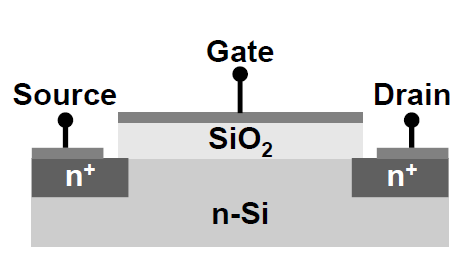
\includegraphics[width=0.35\linewidth]{Kapitel/Kap06/VerarmungNKanalSchnitt}
		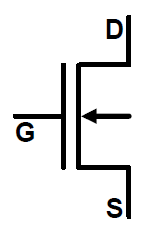
\includegraphics[width=0.125\linewidth]{Kapitel/Kap06/VerarmungNKanalSchaltsymbol}
		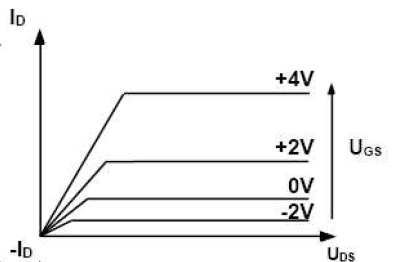
\includegraphics[width=0.325\linewidth]{Kapitel/Kap06/VerarmungNKanalKennlinie}
		
		\textbf{P-Kanal Verarmungstyp:}
		\newline
		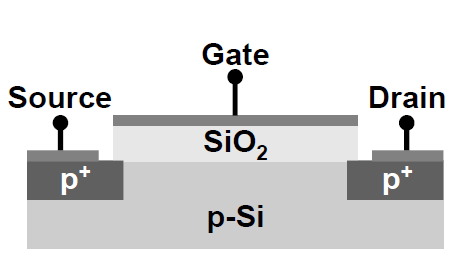
\includegraphics[width=0.35\linewidth]{Kapitel/Kap06/VerarmungPKanalSchnitt}
		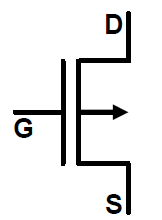
\includegraphics[width=0.125\linewidth]{Kapitel/Kap06/VerarmungPKanalSchaltsymbol}
		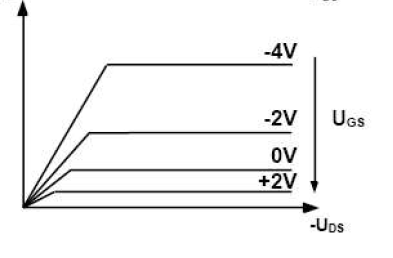
\includegraphics[width=0.325\linewidth]{Kapitel/Kap06/VerarmungPKanalKennlinie}
		
		\textbf{N-Kanal Anreicherungstyp:}
		\newline
		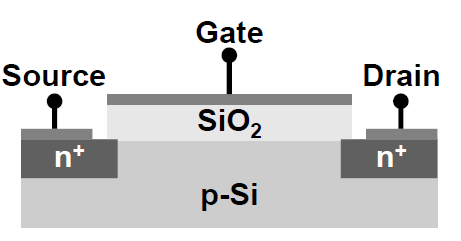
\includegraphics[width=0.35\linewidth]{Kapitel/Kap06/AnreicherungNKanalSchnitt}
		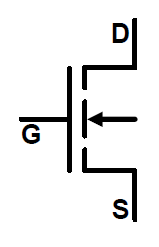
\includegraphics[width=0.125\linewidth]{Kapitel/Kap06/AnreicherungNKanalSchaltsymbol}
		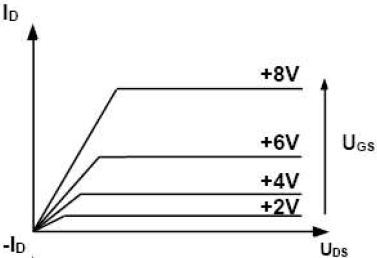
\includegraphics[width=0.325\linewidth]{Kapitel/Kap06/AnreicherungNKanalKennlinie}
		
		
		\textbf{P-Kanal Anreicherungstyp:}
		\newline
		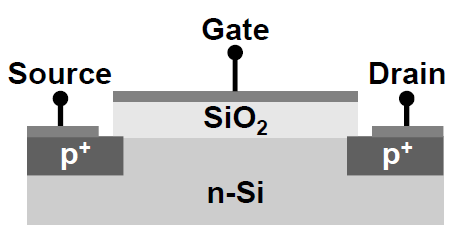
\includegraphics[width=0.35\linewidth]{Kapitel/Kap06/AnreicherungPKanalSchnitt}
		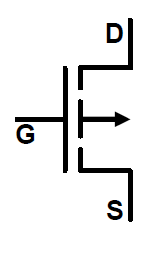
\includegraphics[width=0.125\linewidth]{Kapitel/Kap06/AnreicherungPKanalSchaltsymbol}
		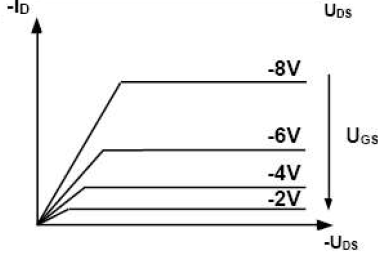
\includegraphics[width=0.325\linewidth]{Kapitel/Kap06/AnreicherungPKanalKennlinie}
		
		 

	\subsubsection{Ausgangs- und Transferkennlinien}
		Die Ausgangskennlinie des MOS-Transistors unterteilt sich in Sperrbereich, linearer Bereich (Triodenbereich) und Sättigungsbereich

		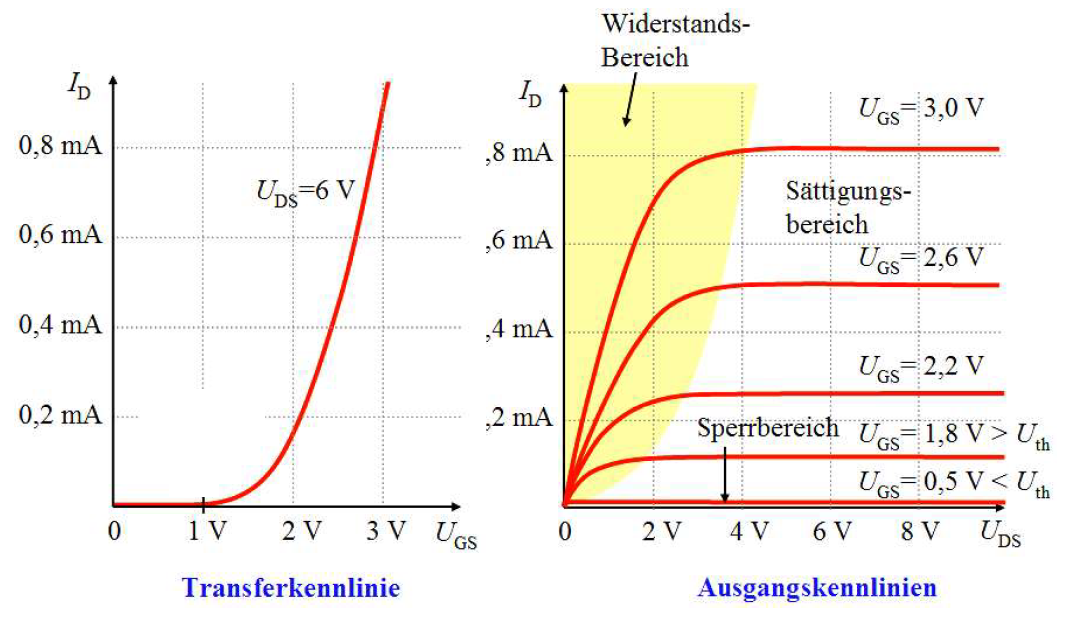
\includegraphics[width=0.8\linewidth]{Kapitel/Kap06/TransferundAusgangskennlinie}
		Durch zunehmend Spannungsabfall im Kanal bildet sich eine Sperrschicht. Es kommt zur Abschnürung des Kanals, zum Pinch-Off/Sättigung: Strom steigt nicht mehr an bei Erhöhung von $U_{DS}$
		\newline
		Ab hier beginnt der Sättigungsbreich.
		\newline
		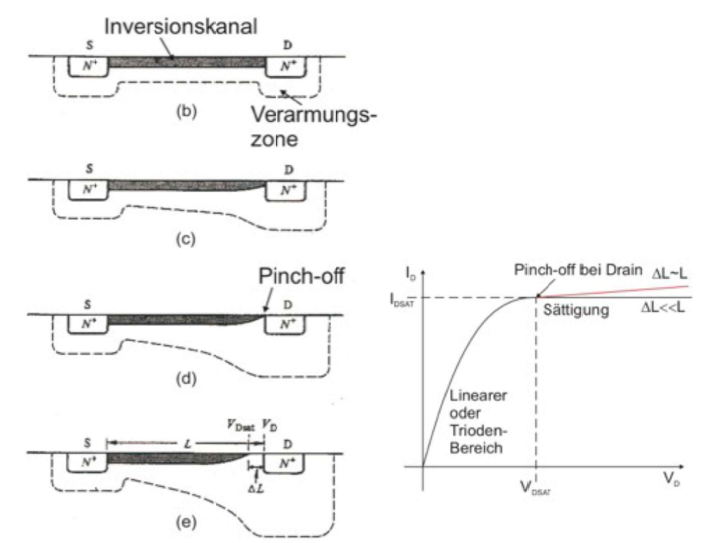
\includegraphics[width=0.6\linewidth]{Kapitel/Kap06/PinchOfff}
		\newline
		Die Steilheit im Linearen Bereich berechnet sich folgendermaßen: 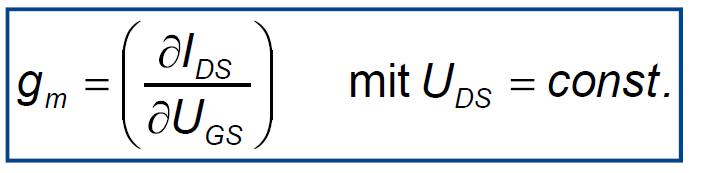
\includegraphics[width=0.3\linewidth]{Kapitel/Kap06/gm}
		\begin{figure}
			\centering
			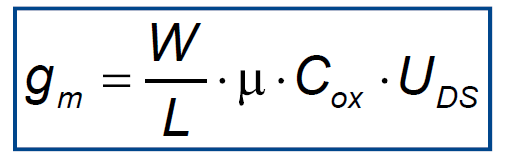
\includegraphics[width=0.3\linewidth]{Kapitel/Kap06/gm1}
			\caption{}
			\label{fig:gm1}
		\end{figure}
\subsection{HEMT}	
	III-V high-electron-mobility transistor (HEMT) oder auch MODFET wird für Hochfrequenzanwendungen verwendet.
	
	\begin{center}
		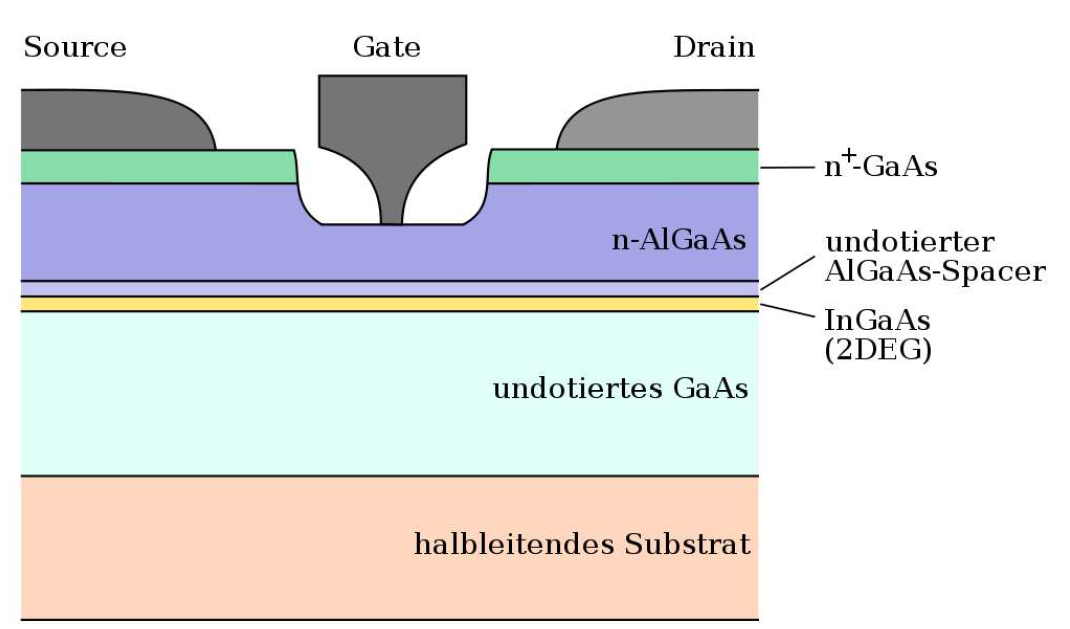
\includegraphics[width=0.4\linewidth]{Kapitel/Kap06/HEMT}
	\end{center}
	
	\todo{Pinzip noch einmal genauer durchsprechen. Ich habe das nicht merh ganz auf die Reihe bekommen}	
\subsection{Anwendungen von MOS-Transistoren}
	Grundprinzip: Kombination von p-Kanal- und n-Kanal-FETs. Durch die gleiche Steuerspannung jeweils zweier komplementärer Transistoren (einmal n-Kanal, einmal p-	Kanal) sperrt immer genau einer, und der andere ist leitend.
	\begin{center}
		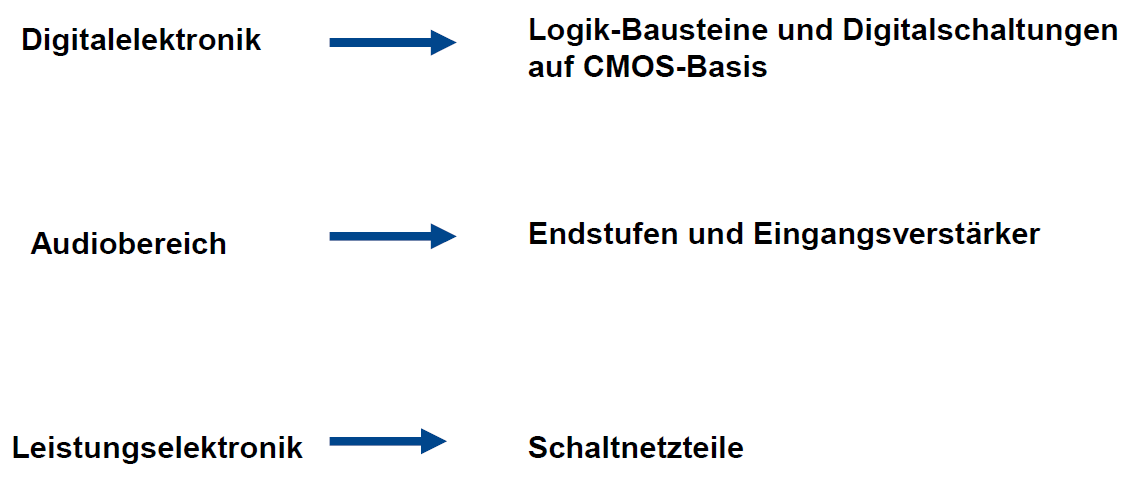
\includegraphics[width=0.7\linewidth]{Kapitel/Kap06/Anwendung}
	\end{center}
\begin{center}
	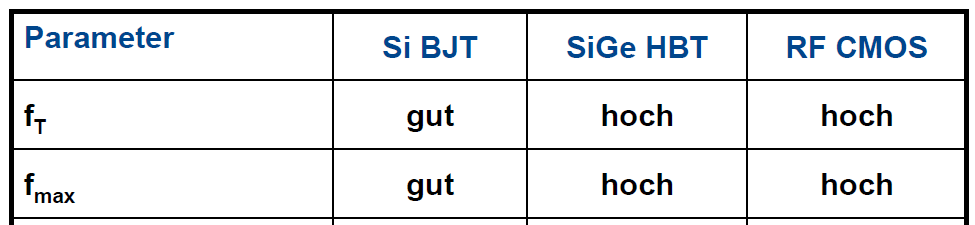
\includegraphics[width=0.7\linewidth]{Kapitel/Kap06/Hochfrequenzanwendungen}
\end{center}

	
	\subsubsection{Vor- und Nachteile}
	\textbf{Vorteile:}
	\newline		
	\begin{itemize}
		\item Der Spannungshub zwischen den beiden logischen 	Spannungsniveaus entspricht der vollen 	Versorgungsspannung		
		\item In jedem der beiden Zustände fließt praktisch kein Strom, da immer ein Transistor ausgeschaltet ist => Statische Verlustleistung ist sehr gering 	
		\item Scharfer Übergang zwischen den logischen Zuständen
	\end{itemize}
	\textbf{Nachteil:}
	\newline		
	\begin{itemize}
		\item Nur beim Schaltvorgang fließt ein signifikanter Strom => Dynamische Verlustleistung
		\item	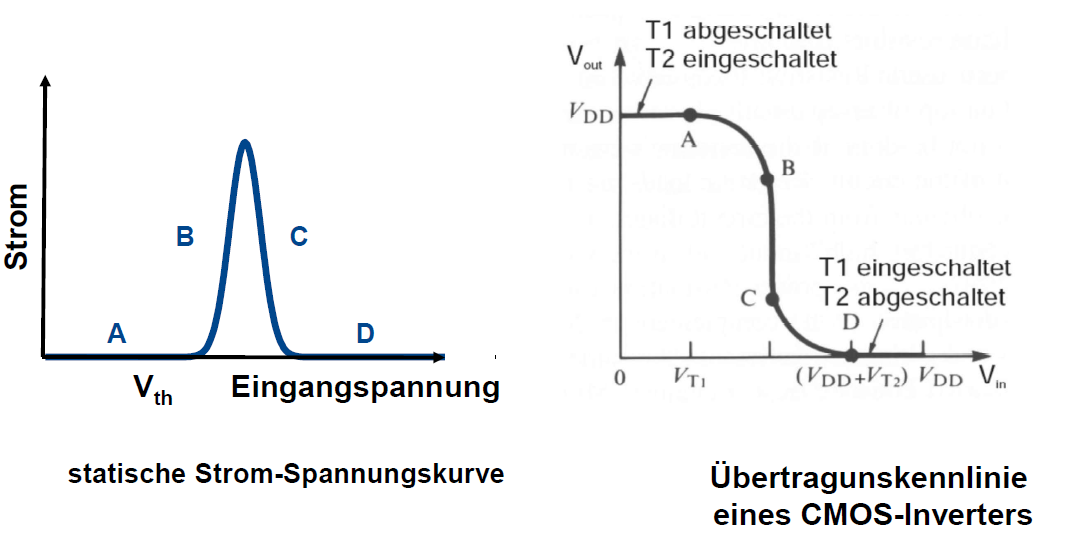
\includegraphics[width=0.4\linewidth]{Kapitel/Kap06/Nachteil}
		
	\end{itemize}
		

	
	\subsubsection{Funktionsprinzip eines CMOS-Inverter}
	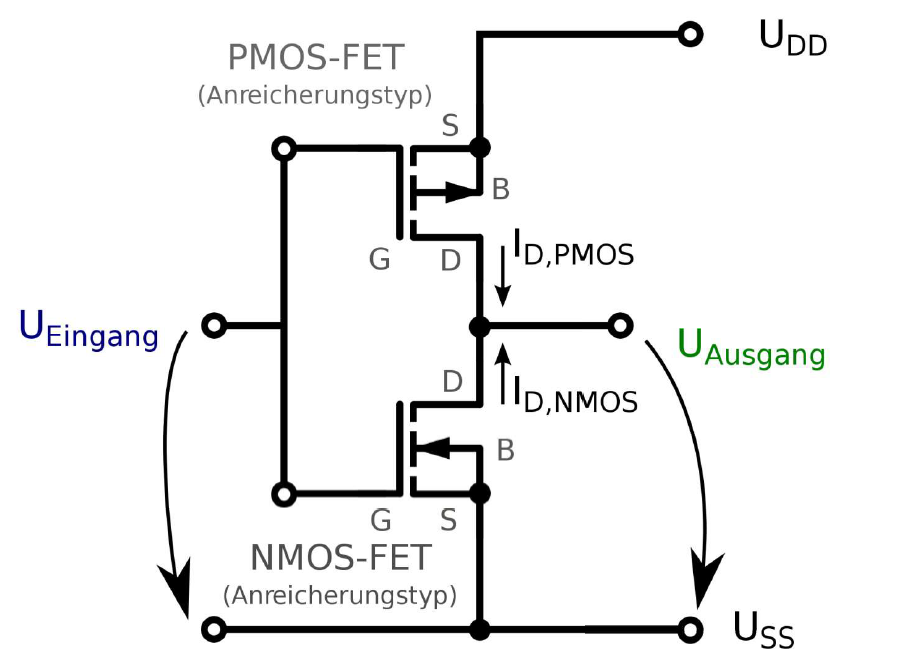
\includegraphics[width=0.5\linewidth]{Kapitel/Kap06/CMOSInverter}
	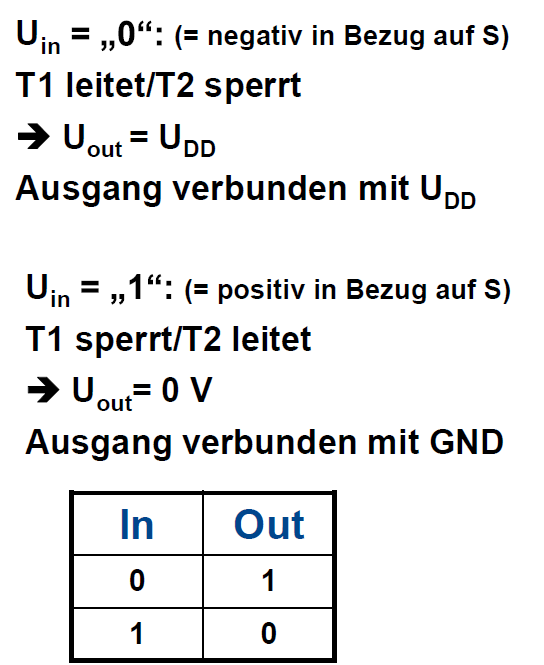
\includegraphics[width=0.4\linewidth]{Kapitel/Kap06/CMOSInverter1}
	\begin{center}
		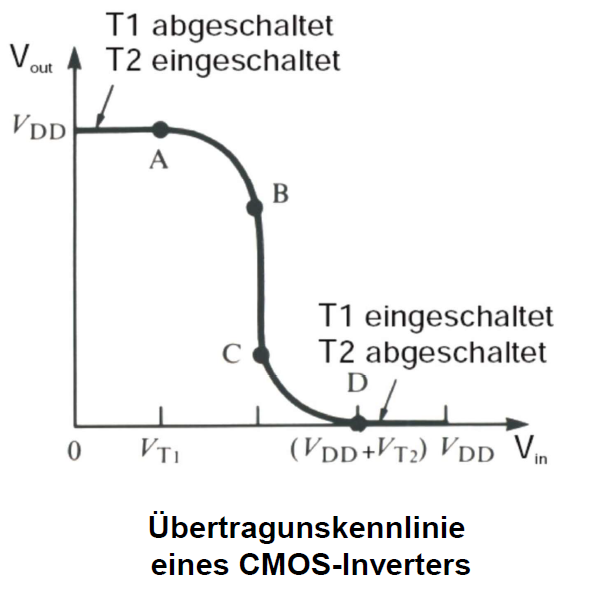
\includegraphics[width=0.3\linewidth]{Kapitel/Kap06/CMOSInverter2}
	\end{center}
	
	


\todo{Fragen aus Own Clowd zuordnen}
\todo{Gruppenübungs-Inhalte ergänzen}